\documentclass[border=10pt]{standalone}

\usepackage{tikz}
\usepackage{tikzsymbols}
\usetikzlibrary{calc,patterns,shapes.geometric}

\def\centerarc[#1](#2)(#3:#4:#5){\draw[#1] ($(#2)+({#5*cos(#3)},{#5*sin(#3)})$) arc (#3:#4:#5);}

\begin{document}
	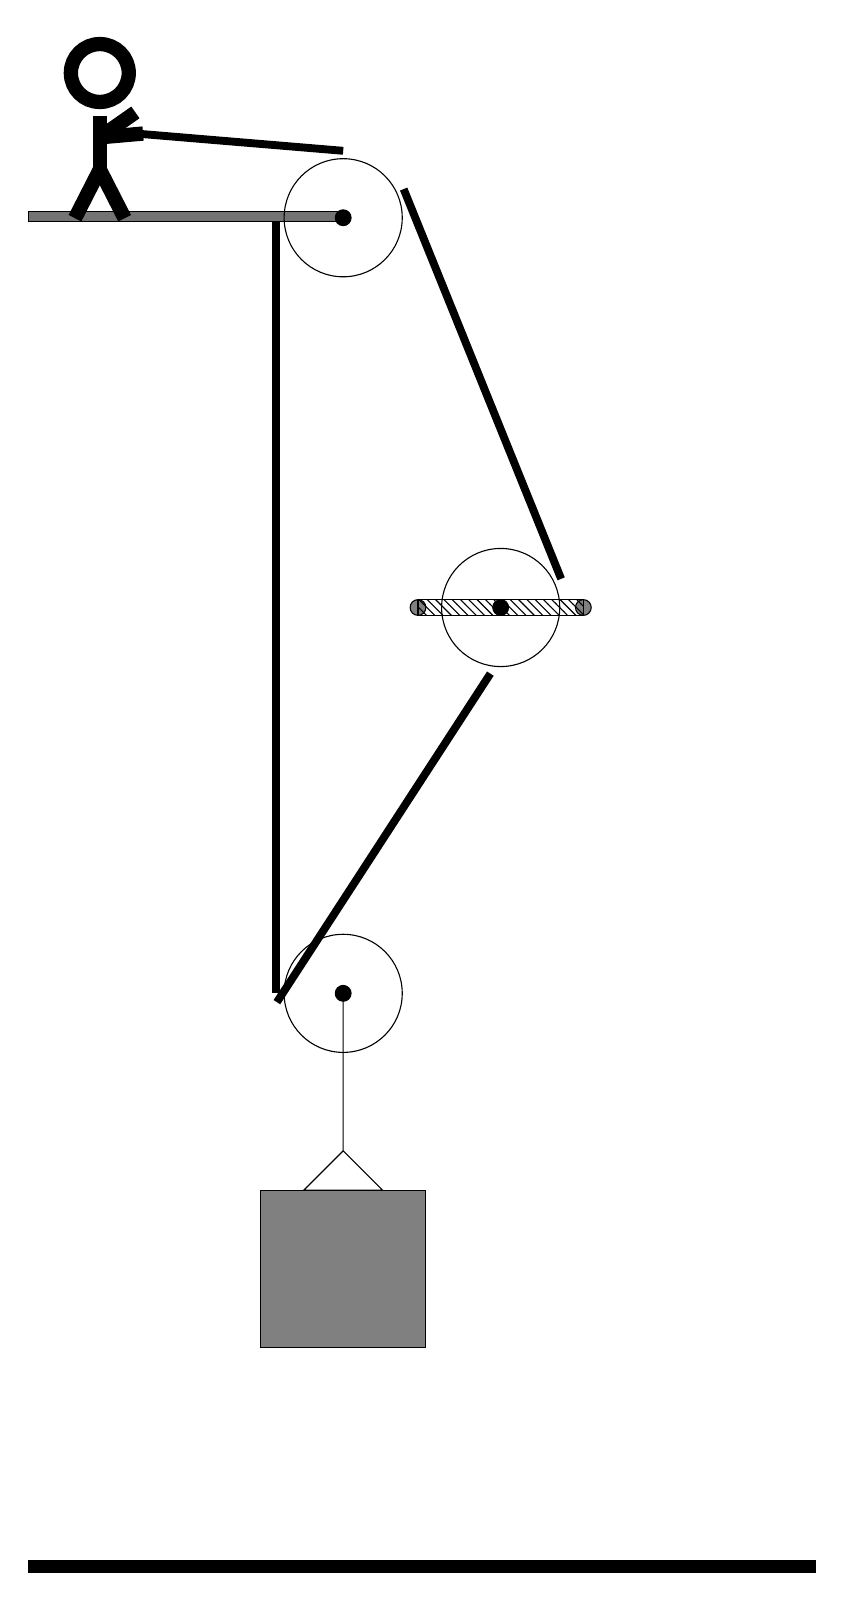
\begin{tikzpicture}
		%%%%% START %%%%%
		\draw[fill=black!55] (-2, 14) rectangle (2, 14.125);
		
		\draw (2, 4.2) circle (0.75);
		\draw[fill=black] (2, 4.2) circle (0.1);
		
		\draw (2, 14.05) circle (0.75);
		\draw[fill=black] (2, 14.05) circle (0.1);
		
		\draw[fill=white](4, 9.1) circle (0.75);
		\draw[fill=black] (4, 9.1) circle (0.1);
		\draw[fill=black!50] (2.95, 9.1) circle (0.1);
		\draw[fill=black!50] (5.05, 9.1) circle (0.1);
		\draw[pattern=north west lines, pattern color=black] (2.95, 9.2) rectangle (5.05, 9.0);
		
		\draw (2, 4.2) -- (2, 2.2) -- (1.5, 1.7) -- (2.5, 1.7) -- (2, 2.2);
		\draw[fill=black!50] (0.95, 1.7) rectangle (3.05, -0.3);
		
		\draw[line width=1mm] (1.15, 14) -- (1.15, 4.2);
		\centerarc[line width=1mm](2, 4.2)(180:330:0.85);
		\draw[line width=1mm](1.158, 4.088) -- (3.869, 8.26);
		\centerarc[line width=1mm](4, 9.1)(390:325:0.85);
		\draw[line width=1mm](4.768, 9.464) -- (2.768, 14.414);
		\centerarc[line width=1mm](2, 14.05)(30:90:0.85);
		\draw[line width=1mm](2, 14.9) -- (-1, 15.15);
		
		\node at (-1, 15.15) {\Strichmaxerl[10][-175][35]};
		
		\draw[fill=black] (-2, -3) rectangle (8, -3.15);
		%%%%% END %%%%%
	\end{tikzpicture}
\end{document}